% For tracking purposes - this is V3.1SP - APRIL 2009

\documentclass{acm_proc_article-sp}

\usepackage{graphicx}
\usepackage{qtree}
\usepackage{alltt}
\renewcommand{\ttdefault}{txtt}

\usepackage{etoolbox}
\makeatletter
\patchcmd{\maketitle}{\@copyrightspace}{}{}{}
\makeatother

\begin{document}

\title{Movelist Learning System}
\subtitle{[Applying Genetic Algorithms to Automate Development of Balanced Turn-Based Combat Mechanics in Role-Playing-Games]}


\numberofauthors{2} 

\author{
% 1st. author
\alignauthor
Austin Cory Bart\\
       \affaddr{Virginia Tech}\\
       \email{acbart@vt.edu}
% 2nd. author
\alignauthor
K. Alnajar\\
       \affaddr{Virginia Tech}\\
       \email{kar@vt.edu}
\alignauthor
}

\date{24 April 2013}

\maketitle
\begin{abstract}
Video game development is a massive industry, and one of the most popular genres to develop are Role-Playing Games. These games often involve a turn-based combat mechanic, which can be extremely time-consuming to create and balance. In order to automate this process, we designed and applied a Genetic Algorithm to the problem of generating effective movelists. Our results show that although the approach is intrinsically sound, more work is required before the output of the system is ready for real-world use.
\end{abstract}

% A category with the (minimum) three required fields
% TODO: We need to look up the tags for this research area
\category{1.2.1}{ARTIFICIAL INTELLIGENCE}{Applications and Expert Systems --- \textit{games}}

\terms{Genetic Programming}

\keywords{Genetic, Programming, Game, Development} % NOT required for Proceedings

\section{Problem}

Turn-based combat is an extremely common video game mechanic in which players fight computer controlled enemies and other players using a pre-defined set of moves called a \textit{movelist}. One of the most challenging aspects of developing this mechanic is finding a functional and balanced movelist. Moves should take advantage of the capabilities of the system, while still being simple and enjoyable for players. At the same time, the moves must be just complicated enough to ensure that players have a good understanding of the game and their own efficacy in order to develop mastery. Creating a movelist that falls within this criteria is a time consuming task for game developers, as the addition and subtraction of moves requires the entire system to be created and tested iteratively. 

A move is an operation that advances a combat from one state to another. A combat's state is given by a set of \textit{attributes}, numbers that indicate the performance and statistics of the players. Although the names of the attributes vary among game engines, common examples include "Health", "Attack", and "defense". For clarity, we differentiate beteween \textit{primary} attributes --- which determine the outcome of a player's battle --- and \textit{secondary} attributes --- which have no direct impact on the outcome of the battle. "Health" is often treated as a primary attribute, as when one player runs out of health then the game is over. "Attack" and "Defense" are used to calculate how much certain moves affect "Health", but their final value has no impact on the outcome of the game, so they are secondary attributes. Moves can take on a vast number of forms, even in a system with a small number of attributes. This model can accurately describe a wide range of popular games with turn-based combat, such as Pokemon \cite{website:pokemon_calculations}. Although many games follow the model of primary and secondary attributes, imbalanced moves lead to many scenarios where secondary attributes can be completely ignored. This "greedy" approach to combat has players simply spamming their primary-affecting moves until they win combat, requiring little strategy.

\subsection{Prior Work}

The problem of generating movelists is largely novel, with little prior work. However, there is a significant, growing interest in formal game development, a largely hitherto ad-hoc process. Many of these tools have a prescriptive nature, rather than explicitly generating code. McNaughton, et al. \cite{generative_design_patterns}, for instance, describe how Generative Design Patterns can be used by novice programmers to create components of video games.

On the other hand, Artificial Intelligence research has led to tools that can automate the game development process and enable emergent gameplay. Amato and Shani\cite{reinforcement-strategy} applied Reinforcement Learning to develop adapative enemies that operate on a strategic -- as opposed to tactical -- level. Zook and Riedl \cite{dynamic_difficulty} examine dynamic difficulty adjustment for players with varying degrees of game skill. Their paper focuses on challenge tailoring in a role-playing style game using a temporal player model to assist in predicting future strength. This concept proposes a way for games to self-monitor and adapt based on player action. This is similar to the work done by Salge, et al. to develop tactical AIs using Genetic Algorithms\cite{genetic-ai}. The Genetic Algorithm approach was used again in work Hom and Marks\cite{balanced-board-games} to automatically generate balanced board game rules based on popular games such as Reversi and Tic-Tac-Toe. The problem that Hom and Marks overcame was very similar to our problem, except instead of developing an entire game engine, we are only exploring how to develop one key component.

\subsection{Approach}

To simplify the development of turn-based combat engines, we have created a system to automatically generate balanced movelists. The system is targetted to game developers who can tailor the framework to their individual game engine.  When designing our system, we studied the problem space very carefully. Because the state space of movelists is extremely large and has many local maxima, our framework uses a \textit{Genetic Algorithm}. A Genetic Algorithm mimics the natural process of evolution by repeatedly manipulating a population of \textit{phenotypes}. These phenotypes are composed of mutable properties called \textit{genes}. Each new iteration of a population is called a \textit{generation}. A phenotype can be changed via \textit{mutation} - where genes are changed at random - and via \textit{cross-over} - where genes are combined with the genes of another phenotype. A \textit{fitness function} maps the phenotypes to a \textit{utility} -- a real number that indicates that phenotype's value in relation to an "ideal" move. 

We performed a number of experiments with our genetic algorithm in order to develop balanced moves. Many of these experiments were staged as we developed the subroutines of our algorithm, in order to ensure that our implementation was well-designed. Afterwards, we varied a multitude of our system's parameters to measure their effect on the rate of utility growth and maximal utility achieved by our system. As we gathered data, we did additional experiments to evaluate the validity of the results achieved.

\section{Implementation of the Genetic Algorithm}

In our system, the phenotype is a movelist and the genes are the moves that make up the movelist. While designing our system, we explored two different implementations of moves. Additionally, we experimented with a number of fitness functions.

\subsection{Fitness Function}

We based our fitness function on the results of battle simulations between two players.  The two players were computer controlled, basing decisions on the Minimax algorithm (limited to depth five). Each player was given a distinct movelist from which to select actions. The utility of the selected moves in the Minimax algorithm was calculated from how they impacted the primary attributes of each player. 

When a battle simulation completes, we use various statistics from the simulation to calculate the fitness. A number of approaches were tested in determining the overall fitness for a set of moves:

\begin{description}
    \item[Move Usage] In an ideally balanced game, all moves should be used approximately equally. Over the course of a battle, we keep track of all the moves used as a ratio of the total moves used. Then, the standard deviation of these percentages is calculated. A well balanced game - where moves are used evenly - has a low standard deviation, but an unbalanced game will have a high deviation.
    \item[Battle Victory] In a typical game, there should be final victory or outcome between the players. This metric awarded a positive utility for battles that involved a victor and a negative reward for battles that ended in a stalemate.
    \item[Battle length] We believed that a good game should last with in a certain range of turns. This way the battles are neither too short (where one player has an overt advantage) or too long (where neither player is able to gain an advantage). 
    \item[Linearity] In order for a battle to progress smoothly, each player should show a steady decrease in primary attributes, rather than a sudden loss at a single point in the battle. This function looked at the progression of player statistics and gave a high utility for battles where both the players’ progress was a steady decrease in attributes, and a negative utility for sudden or extreme changes in the player attributes.
\end{description}

Preliminary testing revealed the most success with a fitness function solely based on Move Usage and Battle Victory. After analyzing the results from the Linearity metric, we determined that this led to battles where the secondary attributes were underrepresented, which was the antithesis of one of our primary goals. Experiments with Battle Length did not seem to have a serious impact on utility, for reasons unclear. Since we desired consistency in our utility function across all results, during our experiments we did not include Battle Length and Linearity in our utility calculations.

\subsection{Move}

As previously described, a move maps how battle states (represented as vectors of values matching attributes) advance to their next states, via mathematical operations. Figure \ref{move-state-transformation} visually shows this transformation.


\begin{figure}[h!]
    \centering
    \begin{tabular}{ | c | c | c || c | c | c | }
        \hline
        \multicolumn{6}{|c|}{Turn i} \\ \hline
        \multicolumn{3}{|c||}{Player 1} & \multicolumn{3}{|c|}{Player 2} \\ \hline
        Health & Attack & Defense & Health & Attack & Defense \\ \hline
        100 & 10 & 10 & 100 & 10 & 10 \\
        \hline
    \end{tabular}
        \smallskip
        {\large $\downarrow$} Player 1 uses a move to affect Player 2's Health        {\large $\downarrow$}
        \smallskip
    \begin{tabular}{ | c | c | c || c | c | c | }
        \hline
        \multicolumn{6}{|c|}{Turn i+1} \\ \hline
        \multicolumn{3}{|c||}{Player 1} & \multicolumn{3}{|c|}{Player 2} \\ \hline
        Health & Attack & Defense & Health & Attack & Defense \\ \hline
        100 & 10 & 10 & \textbf{70} & 10 & 10 \\
        \hline
    \end{tabular}
    \caption{Representation of a move transforming the state of a battle, directly affecting the vector of attribute values.}
    \label{move-state-transformation}
\end{figure}

\subsection{Function Tree}

We first attempted to represent moves as Abstract Syntax Trees of operators over attributes. Every node in the AST is an \textit{operator}, with zero-arity operators (which yield attributes from the input vector, unmodified) being terminal nodes. Early experiments with \textit{ephemeral nodes} - coded as zero-arity operators that returned a constant value, as opposed to an attribute - led to their inclusion. Figure \ref{example function tree} gives an example of a Function Tree with a binary operator (addition), unary operator (doubling), and two nullary operators (Player 1's Attack attribute and an ephemeral constant). At the top of the tree, the output attribute is shown (Player 2's Health attribute). 

\begin{figure}[h]
    \Tree [.P2-Health [.= [.+ 42 [.double() P1-Attack ]]]]
    \caption{Example of a Function Tree}
    \label{example function tree}
\end{figure}

\subsubsection{Mutation Algorithm}

There are many well-known methods for mutating an AST, so we chose to implement a core subset of them:\cite{genetic_programming}
\begin{description}
    \item[Node Replacement Mutation] A node is selected and replaced with another operator of equal arity.
    \item[Subtree Mutation] A subtree is selected, and is given a new parent. This new, taller subtree replaces the original, increasing the depth of the tree.
    \item[Shrink Mutation] A node is selected and its arity is reduced, decreasing the number of subtrees.
\end{description}

    Preliminary tests of the mutation algorithms revealed that mutation had an undesirably dramatic effect on the structure of the Function Tree. In order to keep mutational changes to a minimum, we refactored the algorithms to only affect terminal and pre-terminal nodes. The result of this change is demonstrated in Figure \ref{mutation-edit-distance-terminal-vs-entire}, which shows the lessened logarithmic relationship between the number of times a tree is mutated and the Edit Distance from its parent.
    
    \begin{figure}[h]
        \centering
        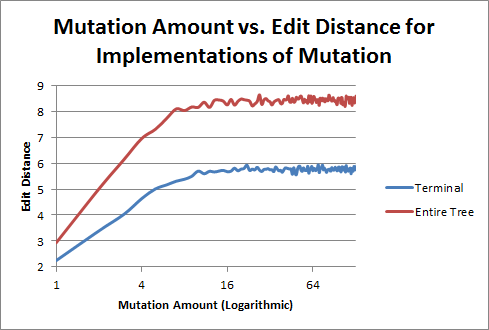
\includegraphics[width=\columnwidth]{./images/mutation-edit-distance-terminal-vs-entire.png}
        \caption{Mutation Amount vs. Edit Distance for Implementations of Mutation}
        \label{mutation-edit-distance-terminal-vs-entire}
    \end{figure}
    
    \subsubsection{Cross-over Algorithm}
    
The problem of crossing over Abstract Syntax Trees is well-established in the literature. We investigated several possible implementations before choosing one based on work by Poli and Langdon \cite{crossover}. Their uniform cross-over algorithm matches common nodes in the two parents trees, starting from the root. When dissimilar parallel nodes (named \textit{Boundary Nodes}) are encountered, a subtree is chosen randomly from the two options. 

Unfortunately, although this implementation was described favorably in the literature, we found that it rarely caused a true combination of the parents, but instead led to one parent being copied wholesale in favor of the other. Figure \ref{cross-over similarity} graphs the result of a 1000 trials where two parents were randomly generated and then crossed with each other. The Percentage Difference from Parent was calculated as the change in edit distance from one parent to the child over the edit distance of the two parents. Ideally, this distributed would be heavily banded around $50\%$; instead, more than 3/5 of the data is at $0\%$ or $100\%$ percent difference (indicating a parent was copied completely).

    \begin{figure}[h]
        \centering
        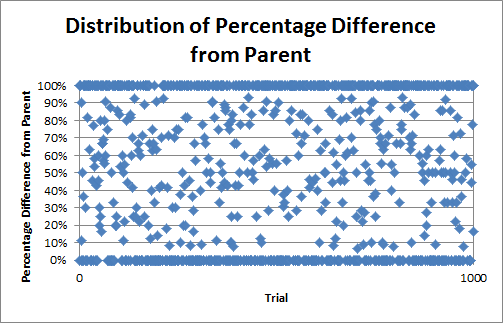
\includegraphics[width=\columnwidth]{./images/dist-perc-diff.png}
        \caption{Distribution of Percentage Difference from Parent in Function Tree Cross-over}
        \label{cross-over similarity}
    \end{figure}
    
    \subsubsection{Validation of Trees}
    
While we performed structural analysis of the our Function Tree implementation, we were doubtful that these structural modifications would have a corresponding impact on the numerical results of the functions. For example, changing a function of the form "Player 1's $1^{st}$ Health + player 2's $1^{st}$ Attack" to use division instead of addition would yield a largely different set of outputs. In order to quantitatively measure the similarity of two functions, we used a two-sample Kolmogorov–Smirnov test. This variant of the KS-test is a non-parametric method for determining if two sets of samples come from the same distribution\cite{ks-test}. 

Because the KS-test expects one-dimensional data, the domain of the inputs (normally multivariate) was restricted from the real numbers to [-100,100], and their cross-product treated as a single input. For example, in a system with one primary attribute and one secondary, the Function Tree would have $$|(100) - (-100)|^4 = 1600000000$$ integer inputs and outputs, following the pattern demonstrated in Figure \ref{ks-test-inputs}.

    \begin{figure}[h]
        \centering
\begin{tabular}{ | c | c | c | c | }
    \hline
    P1 Primary & P1 Secondary & P2 Primary & P2 Secondary  \\ \hline
    -100 & -100 & -100 & -100 \\ \hline
    -100 & -100 & -100 & -99 \\ \hline
    \multicolumn{4}{|c|}{...} \\ \hline
    -100 & -100 & -99 & -100 \\ \hline
    -100 & -100 & -99 & -99 \\ \hline
    \multicolumn{4}{|c|}{...} \\ \hline
    100 & 100 & 100 & 99 \\ \hline
    100 & 100 & 100 & 100 \\ \hline
    \hline
\end{tabular}
        \caption{Input Pattern for the KS-Test}
        \label{ks-test-inputs}
    \end{figure}

To calculate our samples, we strode over the inputs at a moderate pace in order to further reduce the domain. A value of 1 from the test indicates evidence of two completely different functions, whereas a value of 0 indicates evidence of two identical functions.

In our validation trials, we generated two trees randomly, measured their edit distance, and then graphed that metric against the results of a KS-test. Figure \ref{edit distance to ks-test for trees} shows the surprisingly strong correlation between Edit Distance and the KS-Test. Unfortunately, it also demonstrates a weakness of the Function Tree implementation: the values quickly get very high (reaching .4), which means that we expand through the search space extremely quickly even when performing a single mutation.

    \begin{figure}[h]
        \centering
        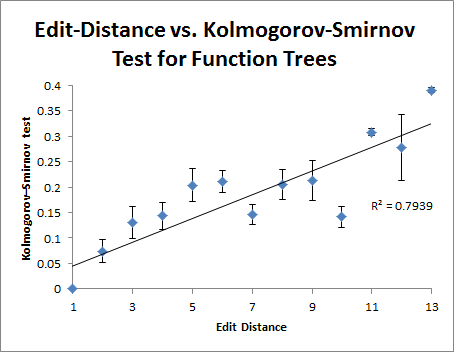
\includegraphics[width=\columnwidth]{./images/edit_distance_vs_ks-test.png}
        \caption{Edit-Distance vs. Kolmogorov-Smirnov Test for Function Trees}
        \label{edit distance to ks-test for trees}
    \end{figure}

	\subsection{Function Vector}
    
Function Trees suffer from a lack of fine-grained state exploration. A single mutation can cause relatively drastic changes to the function. For this reason, we decided to implement and compare an alternative model - functions described as vectors, dubbed Function Vectors. The function vectors map a coefficient to each possible input attribute, with an additional additive constant. When the Function Vector is being evaluated, the current state's values are multiplied by their matching coeffecients, and then summated with the additive constant; Figure \ref{example-function-vector} gives an example of the equation used for evaluating Function Vectors. Due to the fundamental difference between the vector and tree scheme, a different approach was taken for the mutation and cross-over algorithms. 

    \begin{figure}[h]
        \centering
        P2 Health $= (0.1 \times $ P1 Attack $) + (.5 \times $ P2 Attack $) + 5$
        \caption{Example Function Vector}
        \label{example-function-vector}
    \end{figure}
    
    \subsubsection{Mutation Algorithm}
    Function Vectors were mutated by adding a randomly-generated value (limited to a tight range) to a randomly-chosen coeffecient. Because the structure of Function Vector does not change with a mutation, a small percentage of the time the entire FV would be randomly replaced with a completely new move. This ensured that the entire possible state-space for the Vectors was explored.
    
    \subsubsection{Cross-over Algorithm}
    Once again, the constant structure of Vectors made it easy to implement a Cross-over Algorithm. When the parent Vectors had the same output attribute, their coeffecients were individually averaged together. Otherwise, one parent was randomly chosen to be copied wholesale, similar to the way that Function Trees resolved different parents in the extreme case.
    
    \subsubsection{Validation of Vectors}
    To validate the vector mutation function we used the K-S test to look at the difference in changes made by mutation. The results of the K-S test (Figure \ref{fv-mut-vs-ks-test}) showed only a marginal amount of change, which was expected given the limitation imposed on the range of possible coefficients allowed. Although there was no real correlation between the number of times a function was mutated and the results of the K-S test ($R^2 = 0.1394$), this was acceptable given that we were intentionally exploring a smaller state space.
    
    \begin{figure}[h]
        \centering
        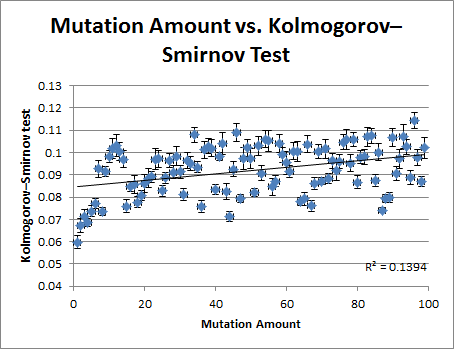
\includegraphics[width=\columnwidth]{./images/fv-mut-vs-ks-test.png}
        \caption{Mutation Amount vs. Kolmogorov-Smirnov Test for Function Vectors}
        \label{fv-mut-vs-ks-test}
    \end{figure}
    
    Validation of the cross-over function for vectors was done through preliminary comparison and analysis of initial battle simulations and iterations. Looking at the utility results when running initial tests showed a correlation between a high cross-over rate and improved utility. These results are demonstrated more explicitly in the next section.
    
    \section{Experiments}
    
    \subsection{Move Generation Experiments}

In order to collect data on the effectiveness of the system and validate the moves, 25 iterations of our Genetic Algorithm were run over a variety of conditions. The base conditions of the algorithm were set as follows, unless manipulated for the purpose of a particular experiment: 
\begin{itemize}
    \item A constant population of 500 movelists
    \item $50\%$ of the new generation would be mutants
    \item $20\%$ of the new generation would be children of crossed-over parents
    \item $30\%$ of the new generation would be top performers from the previous generation
    \item A combat state would have one primary and two secondary attributes.
\end{itemize}

    \subsubsection{Tree vs. Vector}

Both the tree and vector implementations were tested identically in the experiments under the various conditions. The results of the highest utilities of each type of implementation across the iterations were then plotted and analyzed. The vector implementation significantly outperformed the tree implementation across nearly every experiment, with the highest tree utility failing to break a value of 825-utility, whereas the vector implementation reached a 1000-utility score multiple times across various experiments. 

\begin{figure}[h]
    \centering
    
    \caption{Examples of top-performing outputs of the Movelist Learning System}
    \label{example-results}
\end{figure}

    \subsubsection{Mutation Rate vs. Cross-over Rate vs. Parents Retained}

To see the effects of various conditions on the genetic algorithm, these variables were manipulated in multiple experiments, and the effects of these changes can be seen in Figure \ref{utility_experiments}. The results show that for the tree implementation, an equal $20\%$ retention and cross-over rate, with a $40\%$ mutation rate yielded the best results. For the vector implementation, experiments with a high percentage allocated to the mutation and cross-over conditions showed the greatest utility output. The most effective of the conditions was when the mutation and cross-over were equal, with the condition set to $20\%$ retention, $40\%$ mutation and $40\%$ cross-over. This showed a high starting utility and had a moveset with a utility of 1000 after the first iteration.


\begin{figure*}[Ht]
    \centering
    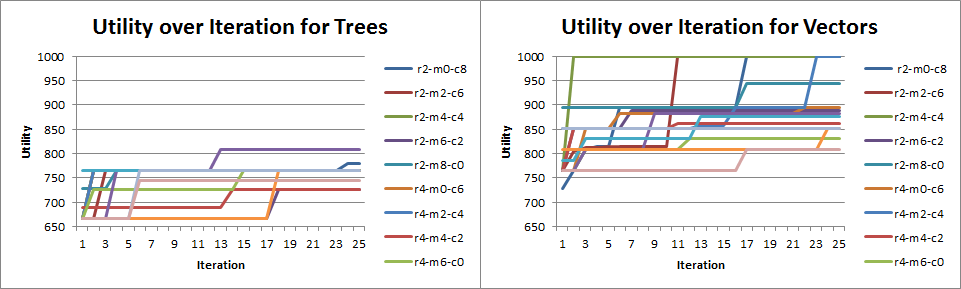
\includegraphics[width=\textwidth,keepaspectratio]{./images/gen-mureco-comparison.png}
    \caption{Maximal Utility over Iterations for Varying Retention, Mutation, and Cross-over Rates}
    \label{utility_experiments}
\end{figure*}

    \subsubsection{Attribute Type Frequencies}

In these tests, we wanted to look at what effect the number of primary and secondary attributes has on the utility of movelists. Attribute type quantities were tested with combinations of 1 to 2 primary attributes and 1 to 3 secondary attributes. Results of these tests can be seen Figure \ref{attribute_frequency_experiments}. For the Tree implementation, the tests have little effect on the utility outcomes, consistently averaging around 750. The results of the Vector tests indicate a stronger impact - tests conducted with a single primary attribute were yielded a higher maximum utility, with a 1000 utility reached in the tests with a single primary attribute, and both two and three secondary attributes. This testing validated the use of the default single primary attribute with two secondary attributes that was used for the attribute type quantities in the other experiments.

\begin{figure*}[Ht]
    \centering
    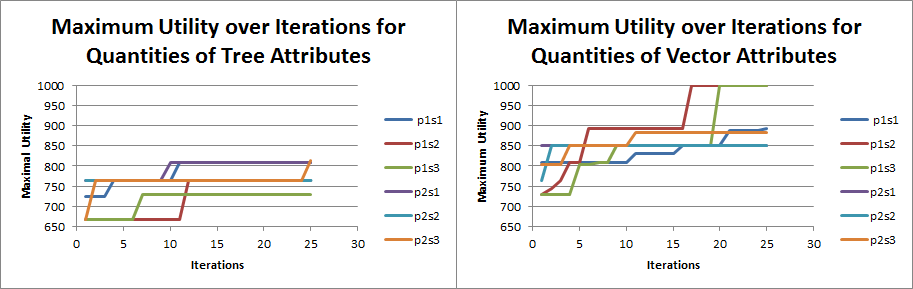
\includegraphics[width=\textwidth,keepaspectratio]{./images/attr_frquency_comparison.png}
    \caption{Maximal Utility over Iterations for Varying Quantities of Attributes}
    \label{attribute_frequency_experiments}
\end{figure*}
    
    \subsection{Validation of Moves}

To look at the effectiveness of some of the 1000-utility moves generated by our solution, we chose to validate the movesets by using a strategic Minimax player, and a nonstrategic (random) or lower level Minimax player to simulate a battle with the moves. With an ideal movelist, the expected outcome of this testing would show that a strategic player would outperform and defeat a less intelligent player.

The results of this testing were unexpectedly negative. In many battle simulations that we analyzed, the lower level Minimax and random players were able to defeat the higher level Minimax player. After looking at the movesets on a case by case basis, it was found that the test results which did not follow the prediction were largely due to an issue in the way moves that affected the primary status of the opponent had been formed. In these cases the losing player often had no move that would be able to reduce a primary attribute of the other player in order to win.
    
    \section{Conclusion}
    
    Although the experiments we conducted on our system produced favorable utilities, our validation metrics indicate that they are not useful for true combat scenarios. The invalidations are mostly likely due to inadequacies of the utility function, which did not take into account that the movelists generated could make it impossible for one or both players to win through strategy. However, we did find that in cases where both players were given a set of moves where each had an effective primary reducing move, the results of the validation experiments were more interesting.
    
    However, the results produced by the system did demonstrate the effectiveness of a Vector-based approach over Trees. Analysis indicates that by limiting the search space, it was easier to find better results and avoid untenable results. It is possible that a hybrid Tree/Vector approach could find a happy medium between the wide-ranging Trees and the narrowing Vectors. In this case, it would be necessary to explore ways to improve the cross-over algorithm for Trees; results indicate that using a high cross-over rate was ineffective compared to high mutation. 
    
    \section{Future Work}

    As indicated by the results of our failed validity tests on the movelists, the most immediate work that needs to be done is a redesign of the utility function calculation. It is possible that given a utility function that takes into account overlooked aspects of the usage in these simulations, the system could generate more practical movelists.

	Another path of research is to abstract the design of the individual moves to provide flexibility for other game engines. In our original design, we proposed a system where every move has a unique function behind it. However, some games use a single formula for every move, and then assign unique attributes on a per-move basis (such as "Base power" or "Accuracy", in addition to player attributes. Supporting game engines such as these might dramatically alter the search space, but could lead to more tenable results.
    
	Finally, we will explore a trending alternative to traditional genetic algorithms called \textit{Novelty Search}, which has been used in research for generating game content dynamically \cite{novelty_search}. The Novelty Search algorithm rewards new behavioral changes in a phenotype, rather than applying a fitness function. By removing the focus on moving towards an objective, which can make it difficult to break out of deceptive local maxima, this algorithm has been shown to be effective for certain problem domains. Given this still inchoate research problem, applying Novelty Search or another variant search algorithm could be a fruitful strategy.
    
%
% The following two commands are all you need in the
% initial runs of your .tex file to
% produce the bibliography for the citations in your paper.
\bibliographystyle{abbrv}
\bibliography{sigproc}  % sigproc.bib is the name of the Bibliography in this case
% You must have a proper ".bib" file
%  and remember to run:
% latex bibtex latex latex
% to resolve all references

%\begin{thebibliography}{1}

% Bibliography goes here

%\end{thebibliography}

%Generated by bibtex from your ~.bib file.  Run latex,
%then bibtex, then latex twice (to resolve references)
%to create the ~.bbl file.  Insert that ~.bbl file into
%the .tex source file and comment out
%the command \texttt{{\char'134}thebibliography}.

\balancecolumns
% That's all folks!
\end{document}